%%
%%  APPENDICES FOR THE CHAPTER 2
%%
\chapter{Some effects for the zip2 synchroniser}
  \section{One of the channels queues is always empty}
TODO
  \section{Brownian motion in unlimited queues}
Explain why the phenomena is observed for $\langle (n_{a} - n_{b})^{2} \rangle$. Explain the similarity of fluctuations of $n_{a} - n_{b}$ the the Brownian motion.

Brownian motion $\langle (n_{a} - n_{b})^{2} \rangle \sim t$, where $n_{a}$ and $n_{b}$ are the number of messages in the channels $a$ and $b$ respectively, and $t$ is time. The average for $(n_{a} - n_{b})$ is taken for 30 experiments. Dependencies close to the Brownian motion $\bar{\Delta l^2} = 2Dt$ take place with the mass diffusivity $D$ as shown in the table below (Коэффициент определен на глаз. По хорошему надо аппроксимировать до прямой: брать среднее от углов наклона для прямых, проведенных через каждую точку). (Probably need to show that the dependency is linear with some statistical criteria like $\chi^{2}$ ?)
  \begin{tabular}{c|c|c|c}
  $m$ & $\sigma$ & $2D$ & $D$\\
  \hline
  $1$ & $2$ & $4$ & $2$\\
  \hline
  $1$ & $1$ & $2$ & $1$\\
  \hline
  $1$ & $0.5$ & $1$ & $0.5$\\
  \hline
  $1$ & $0.25$ & $0.5$ & $0.25$\\
  \hline
  $1$ & $0.125$ & $0.125$ & $0.125$\\ 
  \end{tabular}

Нужно пересчитать эксперимент для $m \neq 1$. Получается что-то похожее на $D = \frac{\sigma}{m^{2}}$. See \ref{fig:brownian}.

It would be good to find $D$ analiticaly!
  \begin{figure}[here]
  \centering
  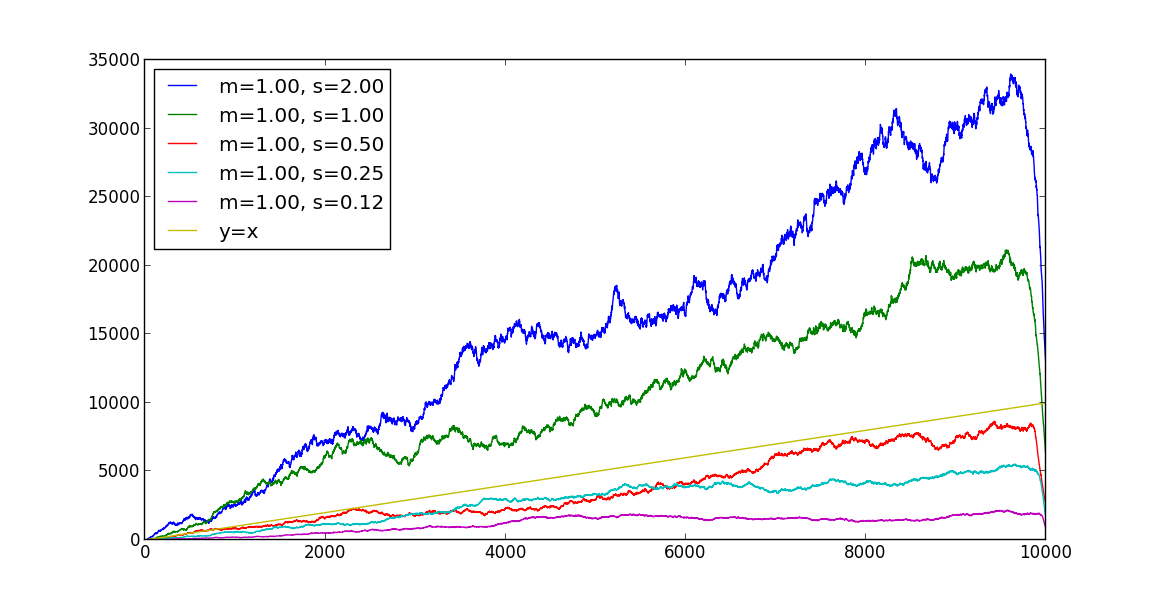
\includegraphics[scale=0.4]{figs/all.png}
  \caption{The evolution of $(n_{a} - n_{b})^{2}$ over time depending on the variance $\sigma$.}
  \label{fig:brownian}
  \end{figure}

